\documentclass[12pt]{article} % use larger type; default would be 10pt

\usepackage{pgfplots}
\usetikzlibrary{calc}
\usetikzlibrary{arrows}
\usetikzlibrary{patterns}
\usetikzlibrary{calc,intersections,through,backgrounds}
\usetikzlibrary{decorations.pathreplacing}
        \usepackage{xcolor} 
        \newcommand\degree[0]{^{\circ}}
        \newcommand\abs[1]{\left|#1\right|}
\usepackage{amsmath}
        \newcommand{\alert}[1]{\boldsymbol{\color{magenta}{#1}}}
        \newcommand{\blert}[1]{\boldsymbol{\color{blue}{#1}}}

\title{Play with TikZ}
\author{Just Us}
%\date{} % Activate to display a given date or no date (if empty),
         % otherwise the current date is printed 

\begin{document}
\maketitle

\section{Chap 5 Section 1}




fig-5-1-3

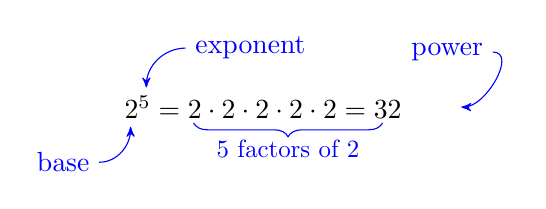
\begin{tikzpicture}
\node[right] at (0,0) {$2^5 = 2\cdot 2\cdot 2\cdot 2\cdot 2=32$};
\coordinate (A) at (.4,.25);
\coordinate (B) at ($ (A)+(.5,.5)$);
\coordinate (C) at (1,-.2);
\coordinate (D) at ($ (C)+(2.4,0)$);
\draw[blue,<-,>=stealth'] (A) to [out=90,in=180] (B) node[right]{exponent};
\draw [blue,decorate,decoration={brace,amplitude=5pt}] (D) -- (C) node [below , midway, yshift=-3,   scale=.9] {5 factors of 2};
\coordinate (E) at (4.8,.7);
\coordinate (F) at (4.4,0);
\draw[blue,<-,>=stealth'] (F) to [out=0,in=0] (E) node[left]{power};
\coordinate (G) at (0.2,-.25);
\coordinate (H) at (-.2,-.7);
\draw[blue,<-,>=stealth'] (G) to [out=270,in=0] (H) node[left]{base};
\end{tikzpicture}
\newline

hp-5-1-40 triangle

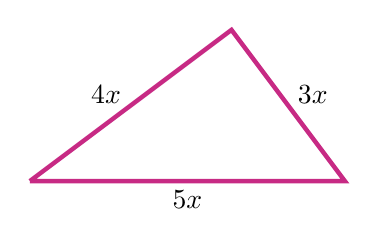
\begin{tikzpicture}
\def\x{0.8};
\coordinate (A) at ({asin(3/5)}:{4*\x});
\coordinate (B) at ({5*\x},0);
\draw[magenta!80!black,ultra thick] (0,0)--(B)--(A)--(0,0);
\node[below] at ({2.5*\x},0) {$5x$};
\node[left, yshift=4] at ($ 0.5*(A)$) {$4x$};
\node[right, yshift=4] at ($ (B) + ({180-acos(3/5)}:{1.5*\x}) $) {$3x$};

\end{tikzpicture}
\newline

hp-5-1-41 triangle

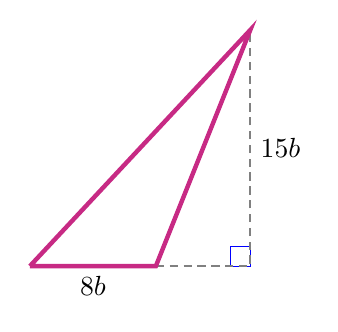
\begin{tikzpicture}
\def\b{0.2};
\coordinate (A) at ({14*\b},{15*\b});
\coordinate (B) at ({8*\b},0);
\coordinate (C) at ({14*\b},0);
\draw[blue] (C) rectangle ++(-.25,.25);
\draw[gray,thick,densely dashed] (B)--(C)--(A) node[right,midway, text=black]{$15b$};
\draw[magenta!80!black,ultra thick] (0,0)--(B)--(A)--(0,0);
\node[below] at ({4*\b},0) {$8b$};
\end{tikzpicture}
\newline

hp-5-1-42 rectangle

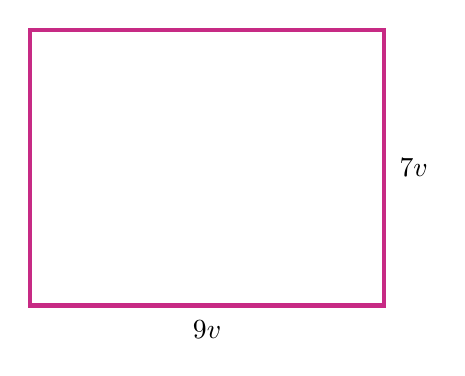
\begin{tikzpicture}
\def\v{0.5};
\coordinate (A) at ({9*\v},{7*\v});
\draw[magenta!80!black,ultra thick] (0,0) rectangle (A);
\node[below, yshift=-2] at ({4.5*\v},0) {$9v$};
\node[right, xshift=2] at ({9*\v},{3.5*\v}) {$7v$};
\end{tikzpicture}
\newline
\section{Chap 5 Section 2}



fig-5-2-1 numberline

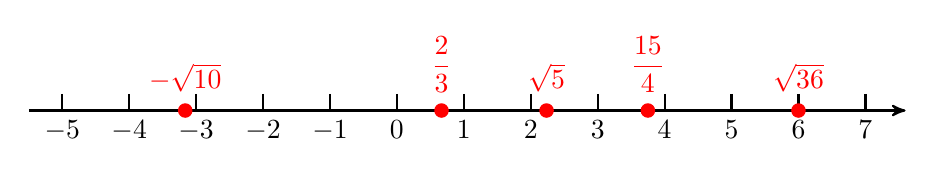
\begin{tikzpicture} [scale=.85]
\draw[black,thick,->,>=stealth'] (-5.5,0)--(7.6,0);
\foreach \x in {-5,-4,...,7}  {
 \draw[black,thick] (\x,.25)--(\x,0) node[below]{$\x$};
}
\filldraw[red] ({-sqrt(10)},0) circle (1mm) node[above, yshift=3] {$-\sqrt{10}$};
\filldraw[red] ({2/3)},0) circle (1mm) node[above, yshift=3] {$\displaystyle\frac{2}{3}$};
\filldraw[red] ({15/4)},0) circle (1mm) node[above, yshift=3] {$\displaystyle\frac{15}{4}$};
\filldraw[red] ({sqrt(5)},0) circle (1mm) node[above, yshift=3] {$\sqrt{5}$};
\filldraw[red] ({sqrt(36)},0) circle (1mm) node[above, yshift=3] {$\sqrt{36}$};
\end{tikzpicture}
\newline



fig-5-2-1 numberline

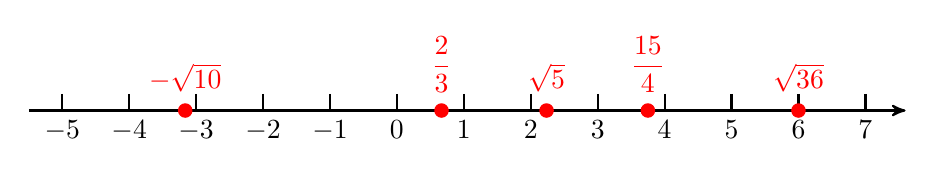
\begin{tikzpicture} [scale=.85]
\draw[black,thick,->,>=stealth'] (-5.5,0)--(7.6,0);
\foreach \x in {-5,-4,...,7}  {
 \draw[black,thick] (\x,.25)--(\x,0) node[below]{$\x$};
}
\filldraw[red] ({-sqrt(10)},0) circle (1mm) node[above, yshift=3] {$-\sqrt{10}$};
\filldraw[red] ({2/3)},0) circle (1mm) node[above, yshift=3] {$\displaystyle\frac{2}{3}$};
\filldraw[red] ({15/4)},0) circle (1mm) node[above, yshift=3] {$\displaystyle\frac{15}{4}$};
\filldraw[red] ({sqrt(5)},0) circle (1mm) node[above, yshift=3] {$\sqrt{5}$};
\filldraw[red] ({sqrt(36)},0) circle (1mm) node[above, yshift=3] {$\sqrt{36}$};
\end{tikzpicture}
\newline
\section{Chap 5 Section 3}


fig-5-3-2 right triangle

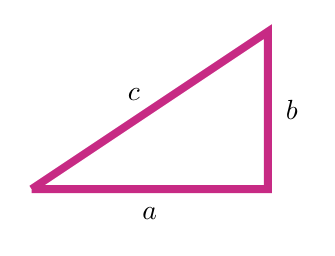
\begin{tikzpicture}
\def\a{3};
\def\b{2};
\draw[magenta!80!black,line width=1mm] (0,0)--(\a,0)--(\a,\b)--(0,0);
\node[below, yshift=-3] at ({\a/2},0) {$a$};
\node[right, xshift=3] at (\a,{\b/2}) {$b$};
\node[above left] at ({\a/2},{\b/2}) {$c$};
\end{tikzpicture}
\newline


hp-5-3-15 triangle

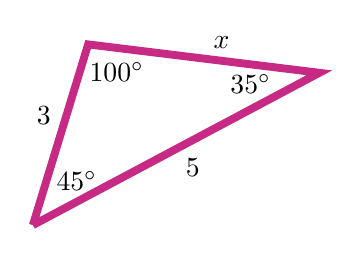
\begin{tikzpicture}
\def\a{28};
\def\b{\a-35};
\def\z{.8};
\def\x{3/sqrt(2)/sin(35)};
\coordinate (A) at ({\a+45}:{3*\z});
\coordinate (B) at (\b:{\x*\z});
\node[above left] at ($ 0.5*(A) $) {$3$};
\node[above right] at ($ (A) + 0.5*(B) $) {$x$};
\node[below right] at ($ 0.5*(A) + 0.5*(B) $) {$5$};
\node[below right, xshift=-3, yshift=-3] at (A) {$100\degree$};
\node[left, xshift=-14, yshift=-4] at ($(A)+(B)$) {$35\degree$};
\node[above right,  xshift=5, yshift=9] at (0,0) {$45\degree$};
\draw[magenta!80!black,line width=1mm] (0,0)--(A)--++(B)--(0,0);
\end{tikzpicture}
\newline


hp-5-3-16 right triangle

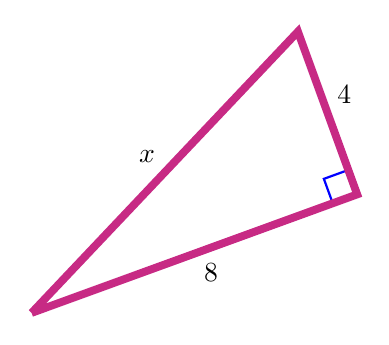
\begin{tikzpicture}
\def\a{20};
\def\b{\a+atan(1/2)};
\def\z{.55};
\coordinate (A) at ({\a}:{8*\z});
\coordinate (B) at ({90+\a}:{4*\z});
\node[below right] at ($ 0.5*(A) $) {$8$};
\node[above right] at ($ (A) + 0.5*(B) $) {$4$};
\node[above left] at ($ 0.5*(A) + 0.5*(B) $) {$x$};
\draw[blue,thick] (A)++({180+\a}:{.6*\z})--++({90+\a}:{.6*\z}) --++({\a}:{.6*\z});
\draw[magenta!80!black,line width=1mm] (0,0)--(A)--++(B)--(0,0);
\end{tikzpicture}
\newline


hp-5-3-17 right triangle

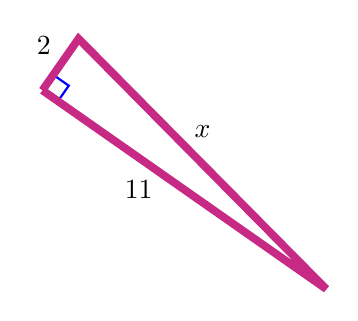
\begin{tikzpicture}
\def\a{55};
\def\b{\a+atan(1/2)};
\def\z{.4};
\coordinate (A) at ({\a}:{2*\z});
\coordinate (B) at ({-90+\a}:{11*\z});
\node[above left] at ($ 0.5*(A) $) {$2$};
\node[above, yshift=6] at ($ 0.5*(A) + 0.5*(B) $) {$x$};
\node[left, xshift=-8] at ($  0.5*(B) $) {$11$};
\draw[blue,thick] (\a:{.6*\z})--++({-90+\a}:{.6*\z}) --++({-180+\a}:{.6*\z});
\draw[magenta!80!black,line width=1mm] (0,0)--(A)--(B)--(0,0);
\end{tikzpicture}
\newline


hp-5-3-18 right triangle

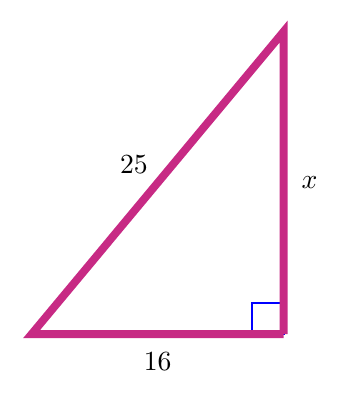
\begin{tikzpicture}
\def\z{.2};
\coordinate (A) at ({-16*\z},0);
\coordinate (B) at (0,{sqrt(625-256)*\z});
\node[below, yshift=-3] at ($ 0.5*(A) $) {$16$};
\node[right, xshift=3] at ($  0.5*(B) $) {$x$};
\node[above left] at ($  0.5*(A)+ 0.5*(B) $) {$25$};
\draw[blue,thick] (0,0) rectangle ++({-2*\z},{2*\z});
\draw[magenta!80!black,line width=1mm] (0,0)--(A)--(B)--(0,0);
\end{tikzpicture}
\newline


hp-5-3-35ans hemisphere

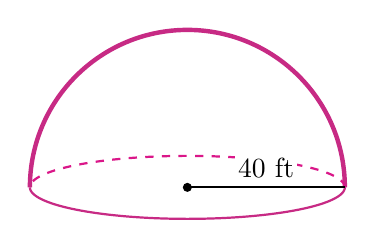
\begin{tikzpicture}
\draw[magenta!80!black, ultra thick] (2,0) arc(0:180:2);
\draw[domain=0:180,variable=\t, smooth, samples=65, magenta!90!black, thick, dashed] plot ({2*cos(\t)}, {.4*sin(\t)});
\draw[domain=0:-180,variable=\t, smooth, samples=65, magenta!80!black, thick] plot ({2*cos(\t)}, {.4*sin(\t)});
\filldraw[black] (0,0) circle (0.5mm);
\draw[black,thick] (0,0)--(2,0) node[above,midway, yshift=2, fill=white, inner sep = 1] {40 ft};

\end{tikzpicture}
\newline



\section{Other stuff}

10 by 10 grid: hp-2-3-12

8 by 8 grid: hp-4-5-17



fig-4-3-ex6a

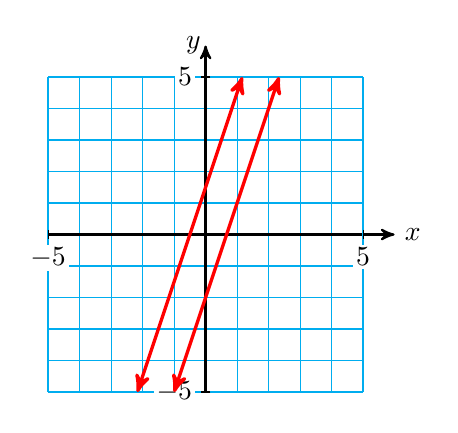
\begin{tikzpicture}[scale=.4]
\def\delx{0};
\draw[cyan] ({-5},-5) grid ({5},5);
\draw[black, thick, ->, >=stealth'] (-5,0)--(6,0) node[right]{$x$};
\draw[black, thick, ->, >=stealth'] (0,-5)--++(0,11) node[left, xshift=2]{$y$};
\foreach \x  in  {-5, 5} {
 \draw[cyan, thick] ({\x},-5) --++(0,10);
 \draw[cyan, thick] ({-5},\x) --++(10,0);
 \draw[black] ({\x},.15) --++(0,-.3) node[below, yshift=-2, fill=white, inner sep=1]   {$\x$};
 \draw[black] ({.15},\x) --++(-.3,0) node[left, xshift=-2, fill=white, inner sep=1]   {$\x$};
}
\draw[red, very thick,<->, >=stealth'] (-1,-5)--(7/3,5);
\draw[red, very thick,<->, >=stealth'] (-13/6,-5)--(7/6,5);
\end{tikzpicture}
\newline

fig-4-3-ex6b
\newline
\end{document}
